\section{Data Quality}
\begin{tcolorbox}[title=The Importance of Validation]
\textbf{Calvin's Dad:} OK Calvin. Let's check over your math homework. \newline
\textbf{Calvin:} Let's not and say we did. \newline
\textbf{Calvin's Dad:} Your teacher says you need to spend more time on it. Have a seat. \newline
\textbf{Calvin:} More time?! I already spent 10 whole minutes on it! 10 minutes shot! Wasted! Down the drain!\newline
\textbf{Calvin's Dad:} You've written here $8+4=7$. Now you know that's not right. \newline
\textbf{Calvin:} So I was off a little bit. Sue me.\newline
\textbf{Calvin's Dad:} You can't \textbf{add} things and come with \textbf{less} than you started with!\newline
\textbf{Calvin:} I can do that! It's a free country! I've got my rights!
\\[-0.6cm]
\begin{flushright}
-- Bill Watterson, \textit{Calvin and Hobbes}, 15-09-1990.
\end{flushright}
\end{tcolorbox}
\noindent
The quality of the data has an important effect on the quality of the results: as the saying goes: ``garbage in, garbage out.''
\newl Data is said to be \textbf{sound} when it has few issues  with 
\begin{itemize}[noitemsep]
\item \textbf{validity} -- are observations sensible, given data type, range, mandatory response, uniqueness, value, regular expressions, etc. (e.g. a value that is expected to be text value is a number, a value that is expected to be positive is negative, etc.)?; 
\item \textbf{completeness} -- are there missing observations (more on this in a subsequent section)?; 
\item \textbf{accuracy and precision} -- are there measurement and/or data entry errors (e.g. an individual has $-2$ children, etc., see  Figure~\ref{fig:targets}, linking accuracy to bias and precision to the standard error)?; \begin{figure*}[t]
\centering
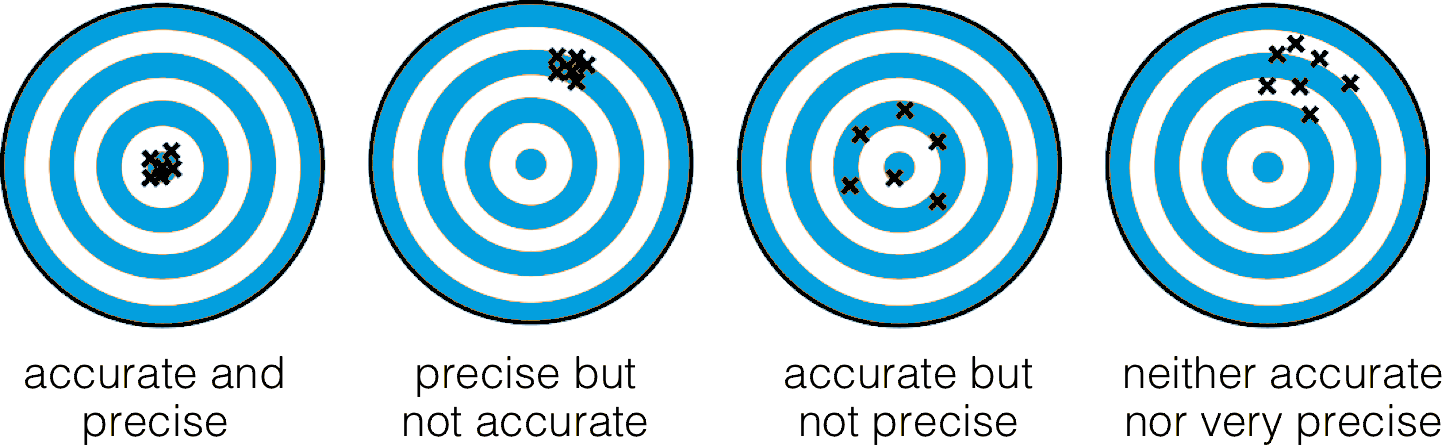
\includegraphics[width=\textwidth]{Images/targets.png}
\caption{\small Accuracy as bias, precision as standard error [author unknown].} \label{fig:targets}\hrule
\end{figure*}
\afterpage{\FloatBarrier}
\item 
\textbf{consistency} -- are there conflicting observations (e.g. an individual has no children, but the age of one kid is recorded, etc.)?, and 
\item \textbf{uniformity} -- are units used uniformly throughout (e.g. an individual is 6ft tall, whereas another one is 145cm tall)?\end{itemize}
\newpage\noindent Finding an issue with data quality after the analyses are completed is a surefire way of losing the client's trust -- check early and often!
\subsection{Common Sources of Error}
If the analysts have some control over the data collection and initial processing, regular data validation tests are easier to set-up. \newl When the analysts are dealing with \textbf{legacy}, \textbf{inherited}, or \textbf{combined} datasets, it can be difficult to recognise errors arising (among others) from \begin{itemize}[noitemsep] \item missing data being given a code; \item `NA`/`blank' entries being given a code; \item data entry errors;\item coding errors;\item measurement errors;\item duplicate entries, and \item heaping (see Figure~\ref{fig:heaping} for an example).\end{itemize} 
\begin{figure*}[t]
\centering
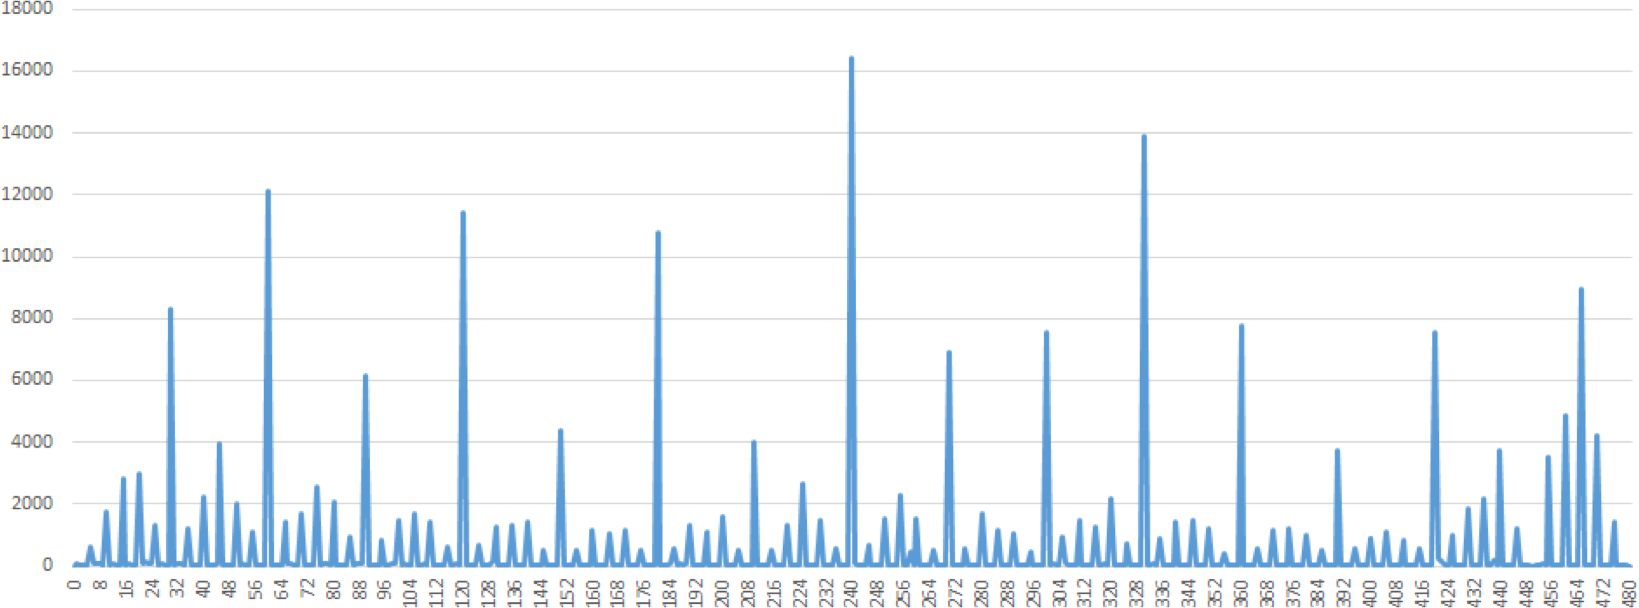
\includegraphics[width=\textwidth]{Images/heaping.png}
\caption[\small An illustration of heaping]{\small An illustration of heaping: self-reported time spent working in a day [personal file]. The entries for 7, 7.5, and 8 hours are omitted. Note the rounding off at various multiples of 5 minutes.}  \label{fig:heaping}
\end{figure*}
%\afterpage{\FloatBarrier}
\subsection{Detecting Invalid Entries}
Potentially invalid entries can be detected with the help of a number of methods: 
\begin{itemize}[noitemsep]
    \item \textbf{univariate descriptive statistics} -- $z-$score, count, range, mean, median, standard deviation, etc.;
    \item \textbf{multivariate descriptive statistics} -- $n-$way tables and logic checks, and \item \textbf{data visualization} -- scatterplot, histogram, joint histogram, etc.
\end{itemize} 
We will not be discussing these methods, but we will point out that univariate tests do not always tell the whole story. 
\begin{center}
    \rule{0.5\linewidth}{.4pt}
\end{center}
Consider, for instance, a medical dataset consisting of 38 patients' records, containing, among others, fields for the \textbf{sex} and the \textbf{pregnancy status} of the patients. A summary of the data of interest is afforded by the frequency counts (1-way tables) shown in Table~\ref{tab:med_data}.
\begin{table*}[t]
       \centering
 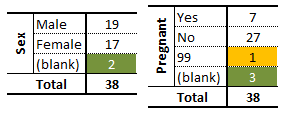
\includegraphics[width=0.48\textwidth]{Images/med_sex_preg}\quad
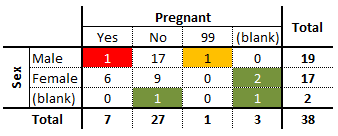
\includegraphics[width=0.48\textwidth]{Images/med_2_way}
\caption{\small Summary data for an (artificial) medical dataset: $1-$way tables (left), $2-$way table (right).}\hrule
        \label{tab:med_data}
\end{table*}
\newpage\noindent 
The analyst can quickly notice that some values are missing (in green) and that an entry has been miscoded as 99 (in yellow). Using only these univariate summaries, however, it is impossible to decide what to do with these invalid entries.\newl The 2-way frequency counts shed some light on the situation, and uncover other potential issues with the data. \par One of the green entries is actually blank along the two variables; depending on the other information, this entry could be a candidate for \textbf{imputation} or outright \textbf{deletion} (more on these concepts in the next section). \par Three other observations are missing a value along exactly one variable, but the information provided by the other variables may be complete enough to warrant imputation. Of course, if more information is available about the patients, the analyst may be able to determine why the values were missing in the first place, although privacy concerns at the collection stage might muddy the waters. \par The mis-coded information on the pregnancy status (99, in yellow) is linked to a male client, and as such re-coding it as `No' is likely to be a reasonable decision (although not necessarily the correct one).\par  A similar reasoning process should make the analyst question the validity of the entry shaded in red -- the entry might very well be correct, but it is important to at least inquire about this data point, as the answer could lead to an eventual re-framing of the definitions and questions used at the collection stage.   
\begin{center}
    \rule{0.5\linewidth}{.4pt}
\end{center}
In general, there is no universal or one-size-fits-all approach -- a lot depends on the \textbf{nature of the data}. As always, domain expertise can help. \newl Remember that a failure to detect invalid entries is \textbf{not a guarantee} that there are in fact no invalid entries in the dataset. It is important not to oversell this step to the client. When only a small number of invalid entries are detected, the general recommendation is to treat these values as  \textbf{missing}, which we discuss presently.
